
%(BEGIN_QUESTION)
% Copyright 2005, Tony R. Kuphaldt, released under the Creative Commons Attribution License (v 1.0)
% This means you may do almost anything with this work of mine, so long as you give me proper credit

The voltage gain of a common-emitter transistor amplifier is approximately equal to the collector resistance divided by the emitter resistance:

$$\includegraphics[width=15.5cm]{i03519x01.eps}$$

Knowing this, calculate the necessary resistance values for the following fixed-value resistor ($R_2$) and potentiometer ($R_1$) to give this common-emitter amplifier an adjustable voltage gain range of 2 to 8:

$$\includegraphics[width=15.5cm]{i03519x02.eps}$$

\vfil 

\underbar{file i03519}
\eject
%(END_QUESTION)





%(BEGIN_ANSWER)

This is a graded question -- no answers or hints given!

%(END_ANSWER)





%(BEGIN_NOTES)

Since we know that the gain of this amplifier is $R_C \over R_E$, we need to choose values for $R_1$ and $R_2$ that will work to give us the correct ratios.

\vskip 10pt

At the minimum gain setting, $R_C$ will be at a minimum.  This means the potentiometer adjusted to zero ohms.  This means the only collector resistance will be $R_2$, making the solution of $R_2$ easy:

$$A_V = {R_C \over R_E}$$

$$2 = {R_2 \over 1500}$$

$$R_2 = 3000 \> \Omega$$

\vskip 10pt

At maximum gain, the potentiometer will be set to its maximum value  Now that we know the value of the fixed resistor $R_2$, we may calculate $R_1$'s resistance quite easily:

$$A_V = {R_C \over R_E}$$

$$8 = {R_1 + 3000 \over 1500}$$

$$12000 = R_1 + 3000$$

$$R_1 = 9000 \> \Omega$$

%INDEX% Electronics review: transistor amplifier circuit

%(END_NOTES)


